\documentclass{beamer}
\usepackage{beamerthemesplit}
\usepackage{booktabs}
\usepackage{graphicx}
\usepackage{transparent}
\usepackage{bbold}
\usepackage[italian]{babel}
\usepackage[utf8x]{inputenc}
\usepackage{listings}
\usepackage{tikz}
\usetikzlibrary{arrows}
\usepackage{amsmath,amsfonts,amssymb}
\usepackage{pgfplots}
\usepackage{scalefnt}
\usepackage{color}
\usepackage{xcolor}
\usepackage{multicol}

\title[mRMR]{mRMR - features selection method}
\institute{
\begin{small}
Corso di Laurea in Informatica Magistrale
\end{small}}
\author{\textbf{Simone Rutigliano}}
\date{\tiny{\today}}

\usebackgroundtemplate{
%    \transparent{0.12}{
     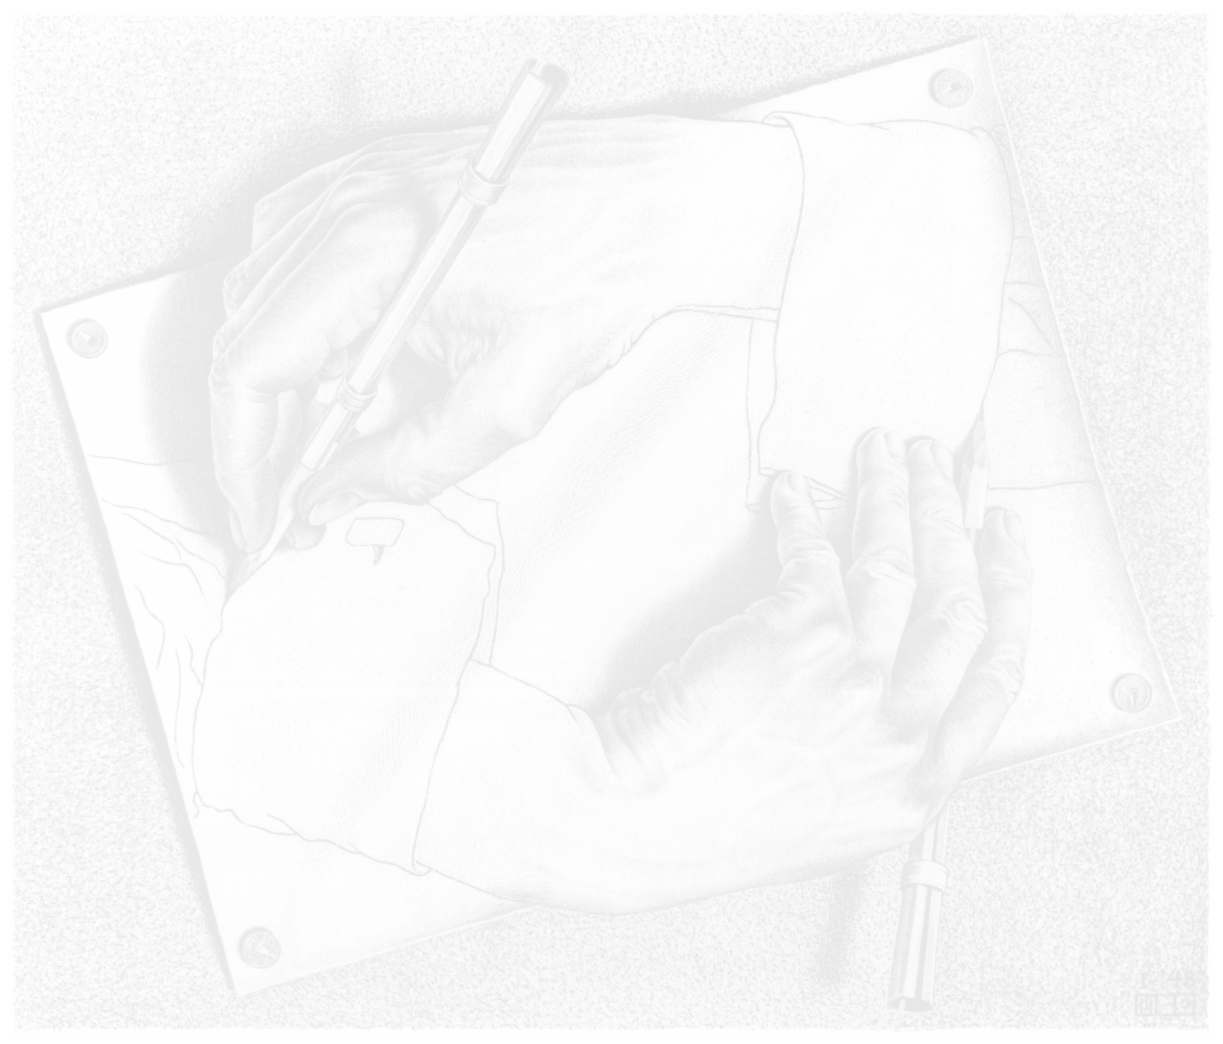
\includegraphics[width=\paperwidth, height=\paperheight]{./figure/theme/escher_hands_tr.png}
%    }
}

%\usetheme{Hannover}
\usetheme{Copenhagen}
\usecolortheme{seahorse}
\usecolortheme{rose}
%\usetheme{Frankfurt}
%\usecolortheme{beetle}

%\useoutertheme[subsection=false]{smoothbars}
%\useoutertheme[subsection=false]{smoothtree}
\useoutertheme{shadow}
\setbeamercovered{dynamic}

\pgfdeclareimage[height=1cm]{logo}{figure/theme/logo}
\logo{\pgfuseimage{logo}}

\begin{document}

%%%%%%%%%%%%%%%%%%%%%%%%%%%%%%%%%%%%%%%%%%%%%%%%%%%%%

\begin{frame}
\maketitle
\end{frame}

%%%%%%%%%%%%%%%%%%%%%%%%%%%%%%%%%%%%%%%%%%%%%%%%%%%%%

\begin{frame}
\frametitle{Outline}
	\begin{multicols}{2}
		\tableofcontents
	\end{multicols}
\end{frame}

%%%%%%%%%%%%%%%%%%%%%%%%%%%%%%%%%%%%%%%%%%%%%%%%%%%%%
\section{Max Dependency}
\subsection{Definizione}
\begin{frame}
	
\end{frame}
\subsection{Formula}
\begin{frame}
	\frametitle{Max Dependency}
	\nocite{Ding:2003:MRF:937976.938050}
	\nocite{Peng05featureselection}
	
	$$ \max D(S,c), D = I(\{x_i,i=1,\dots,m \};c )$$
\end{frame}
\subsection{Problemi}
\begin{frame}
	
\end{frame}

%%%%%%%%%%%%%%%%%%%%%%%%%%%%%%%%%%%%%%%%%%%%%%%%%%%%%

\section{Mutual Information}
\subsection{Definizione}
\begin{frame}
	contenuto...
\end{frame}
\subsection{Formule}
\begin{frame}
	\frametitle{Discrete}
\end{frame}
\begin{frame}
	\frametitle{Continuous}
	$$ I (x;y) = \int \int p(x,y)\log \frac{p(x,y)}{p(x)p(Y)} \mathrm{d}x \mathrm{d}y$$
\end{frame}
\subsection{Problematiche}
\begin{frame}
	contenuto...
\end{frame}

%%%%%%%%%%%%%%%%%%%%%%%%%%%%%%%%%%%%%%%%%%%%%%%%%%%%%
\section{Max Relevance}
\subsection{Definizione}
\subsection{Formule}
\begin{frame}
	\frametitle{Per variabili discrete}
	$$\max D(S,c), D= \frac{1}{|S|} \sum\limits_{x_i \in S} I (x_i;c)$$
\end{frame}
\begin{frame}
	\frametitle{Per variabili continue}
\end{frame}
\subsection{Problematiche}
\begin{frame}
	\frametitle{ridondanza}
	si incorre nel problema della ridondanza
\end{frame}

%%%%%%%%%%%%%%%%%%%%%%%%%%%%%%%%%%%%%%%%%%%%%%%%%%%%%
\section{Min Redundancy}
\subsection{Definizione}
\begin{frame}
	contenuto...
\end{frame}
\subsection{Formule}
\begin{frame}
	\frametitle{Per variabili discrete}
	$$\min R(S), D= \frac{1}{|S|^2} \sum\limits_{x_i,x_j \in S} I (x_i;x_j)$$
\end{frame}
\begin{frame}
	\frametitle{Per variabili continue}
\end{frame}

%%%%%%%%%%%%%%%%%%%%%%%%%%%%%%%%%%%%%%%%%%%%%%%%%%%%%

\section{mRMR}
\subsection{Definizione}
\begin{frame}
	\frametitle{Def}
\end{frame}

\subsection{Formule}
\begin{frame}
	\frametitle{Discrete - MID}
	$$\max \Phi(D,R), \Phi = D - R$$
	dove $D=I(i,h)$ e $R=\frac{1}{|S|}\sum\limits_{j \in S}I(i,j)$
\end{frame}

\begin{frame}
	\frametitle{Discrete - MIQ}
	$$\max \Phi(D,R), \Phi = \frac{D}{R}$$
\end{frame}
\begin{frame}
	\frametitle{Continuous}
	$$ F(g_i,h) = \frac{\frac{\sum\limits_{K}{n_k(\bar{g_k}-\bar{g})}}{K-1}}{\sigma^2}$$
	dove: $\sigma^2=\frac{ \sum\limits_{k}{(n_k-1)\sigma^2_k}}{n-K}$
\end{frame}
\begin{frame}
	\frametitle{Continuous - FCD}
\end{frame}

\begin{frame}
	\frametitle{Continuous - FCQ}
\end{frame}

\subsection{Benefici}
\begin{frame}
	\frametitle{Benefici}
\end{frame}
%%%%%%%%%%%%%%%%%%%%%%%%%%%%%%%%%%%%%%%%%%%%%%%%%%%%%

\begin{frame}{Bibliography}
	\frametitle{References}
	\bibliographystyle{alpha}
	\bibliography{mybib}
\end{frame}
\end{document}
